\documentclass{beamer}
\usetheme{Berlin}
\usecolortheme{dolphin}

\usepackage[T1]{polski}
\usepackage[polish]{babel}
\usepackage[utf8]{inputenc}
\usepackage[T1]{fontenc}
\usepackage[mediumspace,mediumqspace,Grey,squaren]{SIunits}
\usepackage{graphicx}
\usepackage{hyperref}
\usepackage{amsmath}
\usepackage{graphicx}
\usepackage{caption}
\usepackage{subcaption}
\usepackage{geometry}
\usepackage{float}

%\addbibresource{bibliography.bib}

%\setbeamertemplate{bibliography item}{\insertbiblabel}


\graphicspath{ {./images/} }

\begin{document}
\title{Seminarium dyplomowe magisterskie}
\author{Jakub Postępski}
\date{5 czerwca 2019}

\frame{\titlepage}

\section{Zarys pracy magisterskiej}
\begin{frame}{Sterowanie ramieniem robota w obliczu chwytania przedmiotów}

\begin{itemize}
\item Dr inż. Tomasz Winiarski
\end{itemize}

\begin{itemize}
\item Sterowanie siłowe
\item Odczyty wartości z receptorów i możliwość sterowania efektorami
\item Nieznany model chwytanego obiektu
\end{itemize}
\end{frame}


\begin{frame}[allowframebreaks]{Robot usługowy Velma}
\begin{itemize}
\item Dwa manipulatory LWR (sterowanie impedancyjne)
\item Chwytaki Barretta (sztuczna skóra, czujniki siły)
\item Nadgarstkowe czujniki siły i momentu
\item Kinect
\item Stereopara
\item Komputer sterujący
\end{itemize}
\framebreak
\begin{figure}[h]
	\centering
	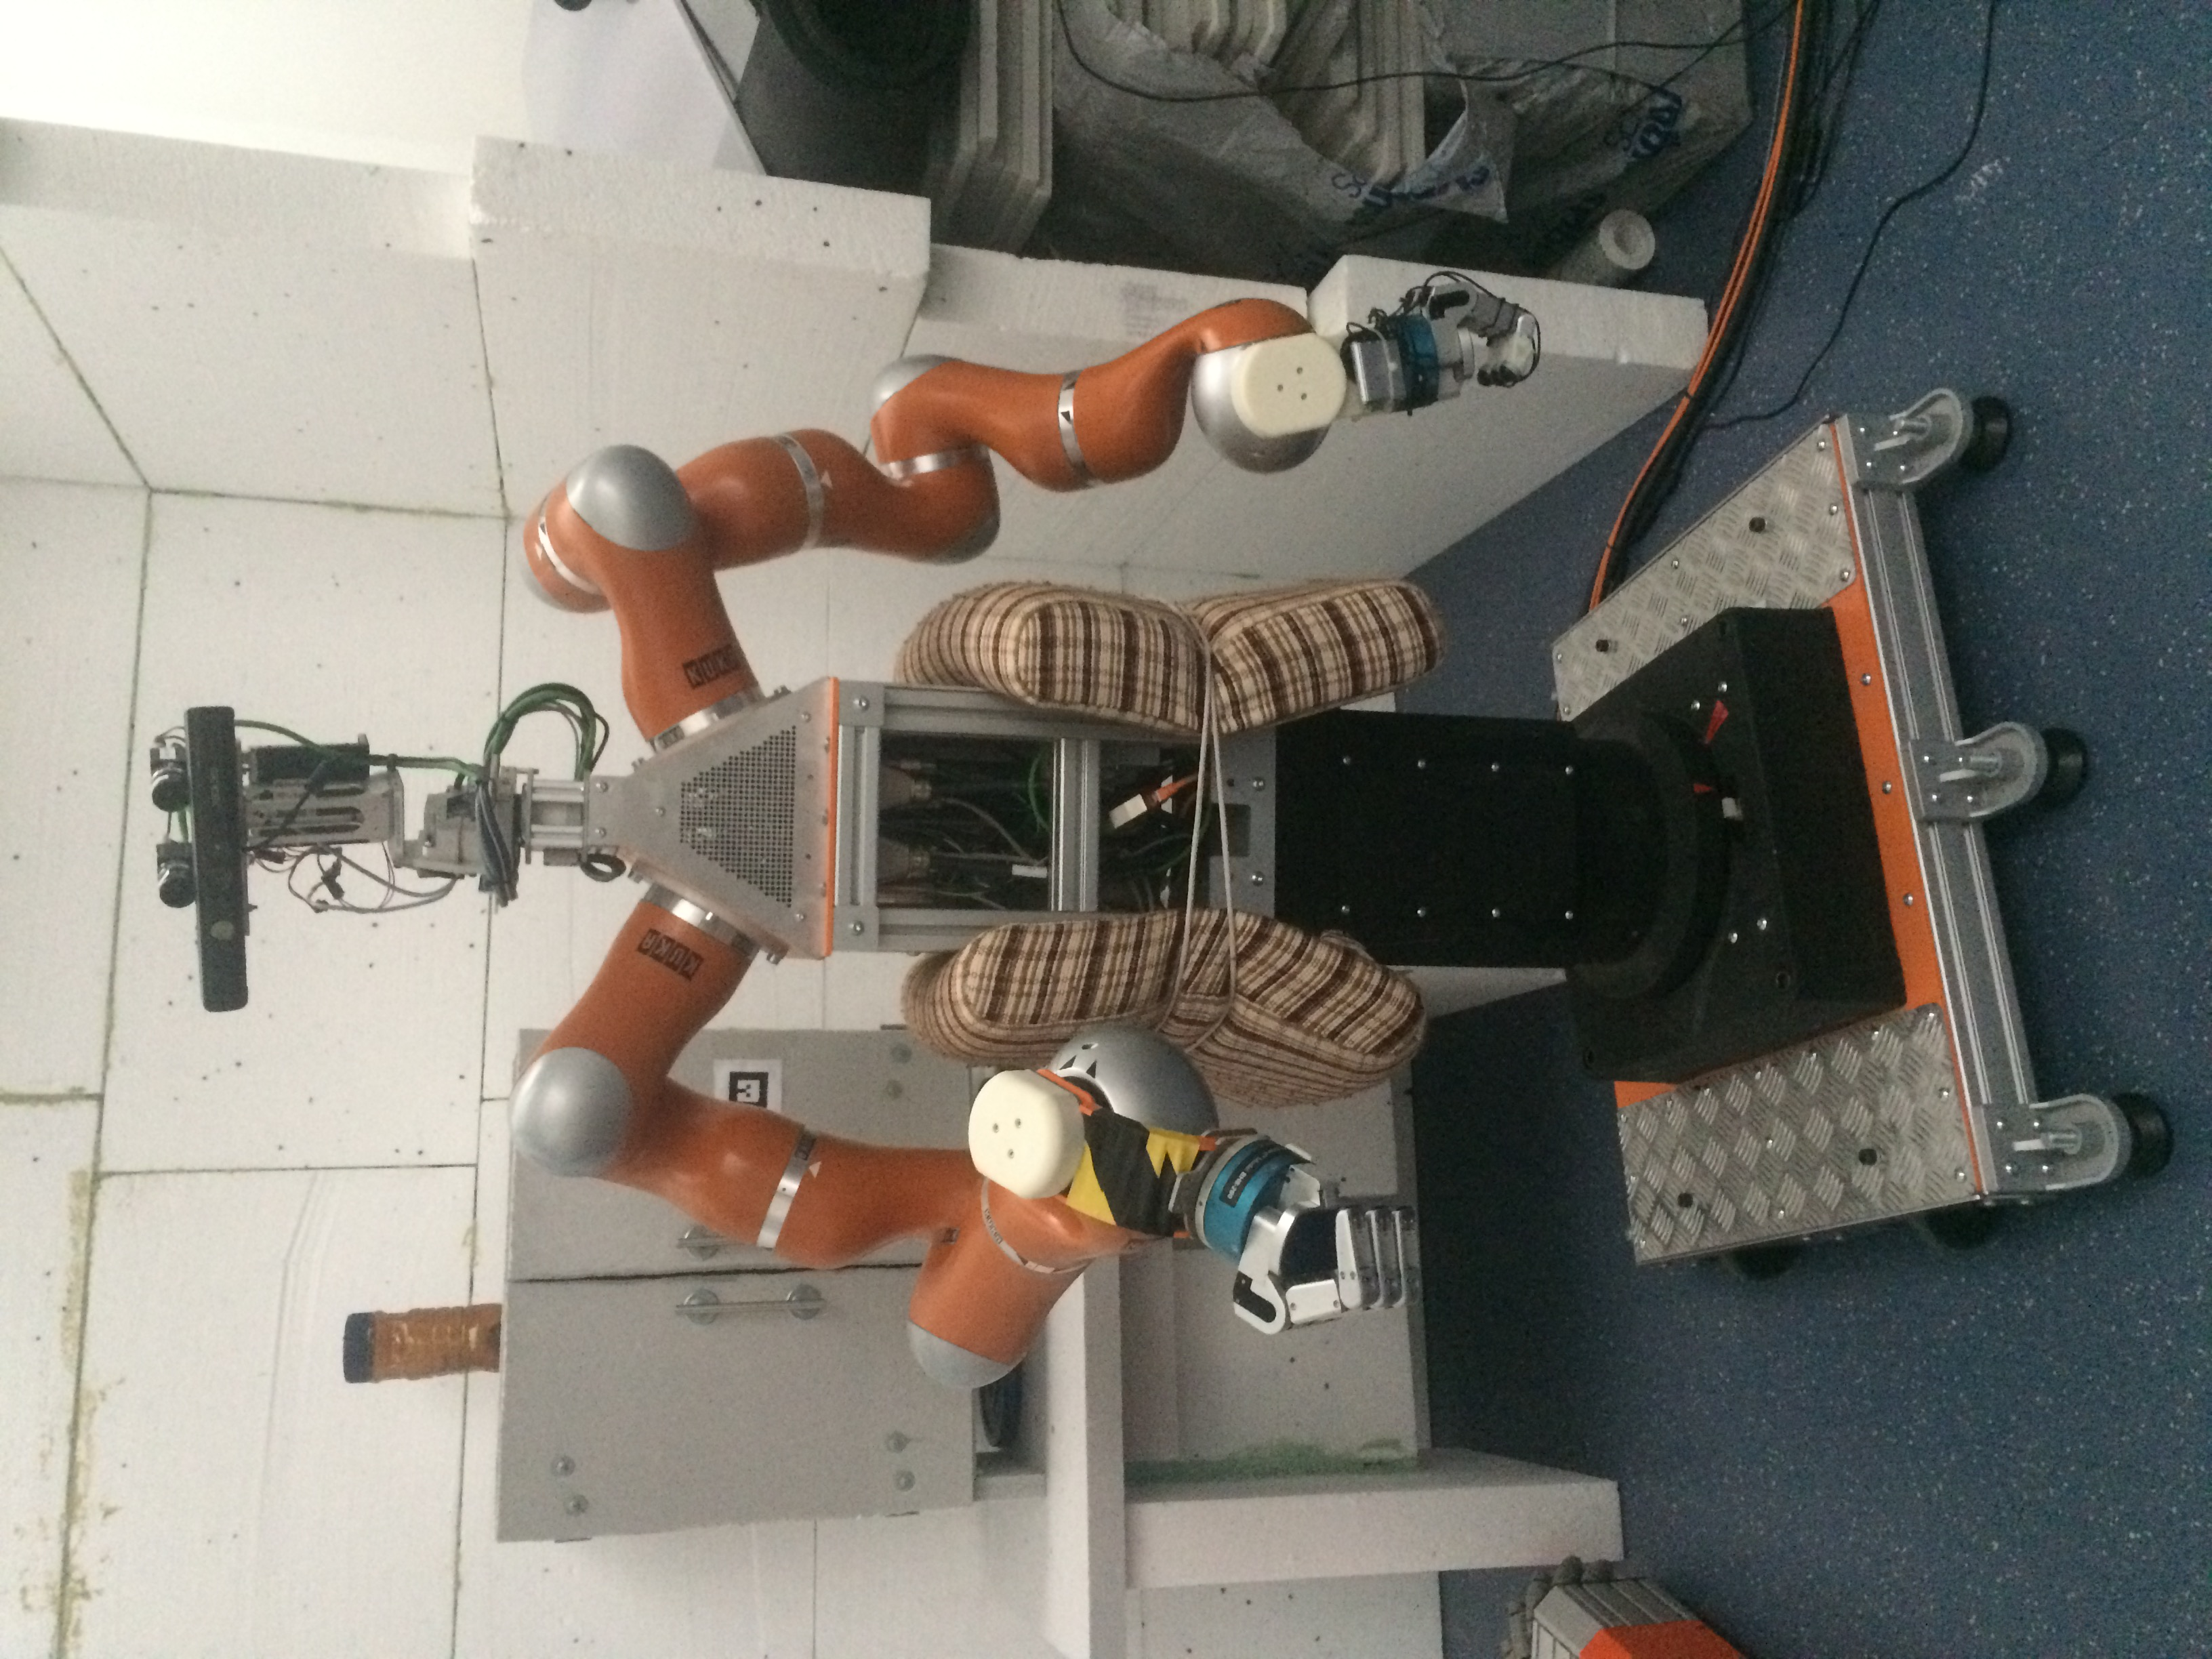
\includegraphics[scale=0.07, angle =-90]{velma1}
\end{figure}

\end{frame}

\begin{frame}[allowframebreaks]{Struktura oprogramowania}


\begin{figure}[h]
	\centering
	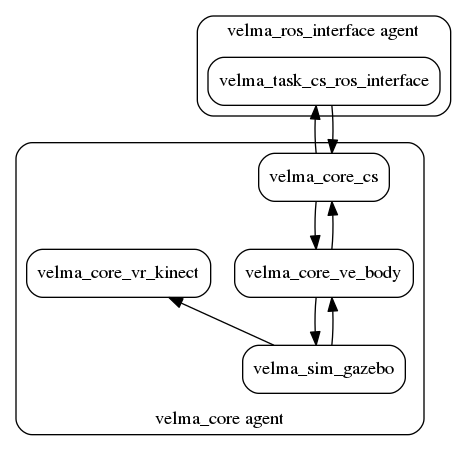
\includegraphics[scale=0.3]{system}
\end{figure}

\framebreak
Częstotliwość pętli sterowania to 500 Hz.

\begin{itemize}
	\item ROS
	\item Orocos
\end{itemize}

Symulator działania z modelem fizyki i symulacją czasu.

\begin{itemize}
	\item Gazebo
	\item Dart
\end{itemize}
\end{frame}

\section{Koncepcja rozwiązania problemu}

	\begin{frame}[allowframebreaks]{Sterowanie impedancyjne}
		\begin{figure}[h]
			\centering
			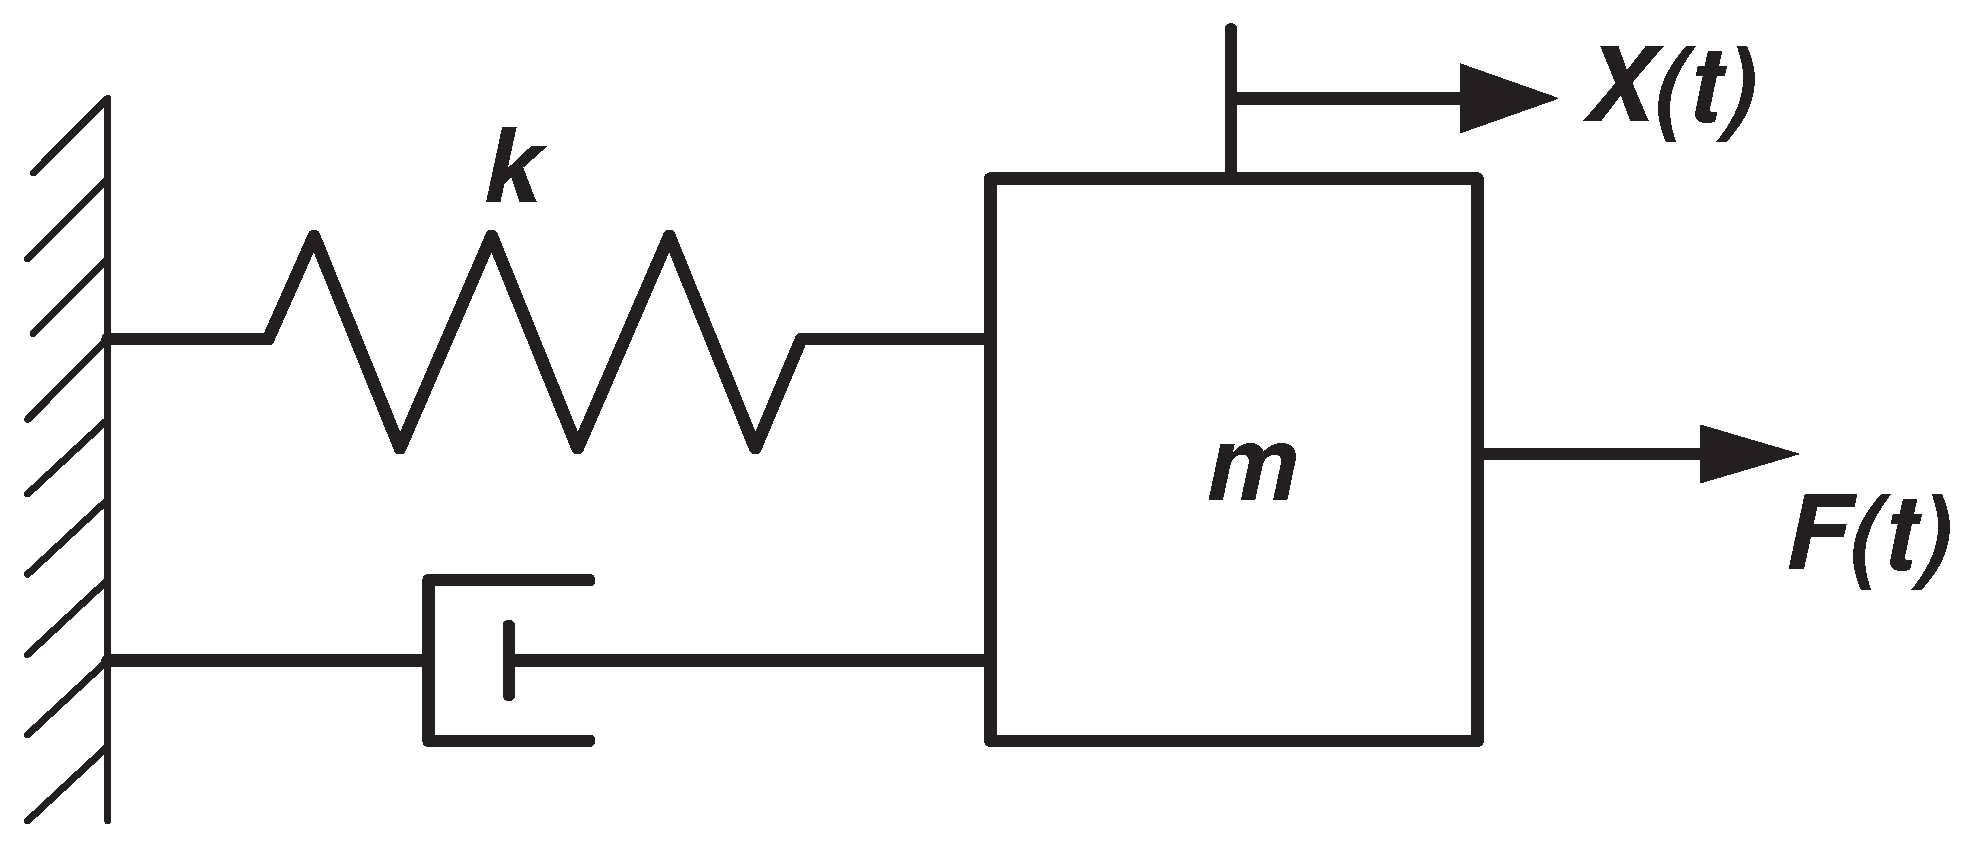
\includegraphics[scale=1.30]{mds}
		\end{figure}

Uproszczone prawo sterowania:
	\begin{equation}
	F = kx + d\dot{x}
	\end{equation}

Prawo sterowania w przestrzeni stawów:
	\begin{equation}
	\tau = K[q_d-q] + D[\dot{q}] + \hat{M}(q)\ddot{q_d} + \hat{c}(q, \dot{q}) + \hat{g}(q) + \hat{h}(q, \dot{q})
	\end{equation}

\begin{itemize}
	\item $\tau$ Moment
	\item $K$ Sprężystość
	\item $D$ Tłumienie
	\item $M$ Macierz inercji
	\item $c$ Siła Coriollisa
	\item $g$ Grawitacja
	\item $h$ Pozostałe siły
\end{itemize}
\end{frame}

\begin{frame}{Model robota}
	Dla członu i-tego mamy:
	\begin{itemize}
		\item Masa $m_i$
		\item Tensor bezwładności $I_{3x3}$ (macierz semisymetryczna)
		\item Macierz inercji $M_{xi 6x6}$
	\end{itemize}
	\begin{equation}
	M_{xi}=
	\begin{bmatrix}
	m_i & 0 & 0 & 0 & 0 & 0 \\
	0 & m_i & 0 & 0 & 0 & 0 \\
	0 & 0 & m_i & 0 & 0 & 0 \\
	0 & 0 & 0 & I_{xx} & I_{xy} & I_{xz} \\
	0 & 0 & 0 & I_{yx} & I_{yy} & I_{yz} \\
	0 & 0 & 0 & I_{zx} & I_{zy} & I_{zz} \\
	\end{bmatrix}
	\end{equation}

	Dla wszstkich członów razem mamy macierz $M(q)$ opisującą inercję w przestrzeni stawów.


	Wniosek: Model chwytanego przedmiotu możemy opisać w ten sam sposób co kolejne człony robota.
\end{frame}

\begin{frame}{Algorytm kompensacji}
	\begin{itemize}
		\item Wykrycie parametrów modelu
		\item Dopisanie odpowiednich momentów do prawa sterowania
	\end{itemize}
\end{frame}

\begin{frame}{Estymacja parametrów}

	Można zastosować optymalizację minimalizującą sumę błędów kolejnych odczytów:
	\begin{equation}
	e(t) = \begin{bmatrix}
	F(t) - \hat{F(t)}\\
	\tau(t) - \hat{\tau(t)}
	\end{bmatrix}
	\end{equation}

	\begin{equation}
	\begin{aligned}
	& \underset{m, M(q)}{\text{min}}
	& & \sum_{t = 1}^{T} || e(t) ||
	\end{aligned}
	\end{equation}

\end{frame}

\begin{frame}[allowframebreaks]{Narzędzia}
	Przestrzenie:
	\begin{itemize}
		\item Stawów
		\item Operacyjna
	\end{itemize}

	\begin{equation}
		\dot{x} = J(q)\dot{q}
	\end{equation}
	\begin{itemize}
	\item $x$ Współrzędne przestrzeni operacyjnej
	\item $q$ Współrzędne przestrzeni stawów
	\item $J$ Jakobian
\end{itemize}
\framebreak

	\begin{equation}
	\tau_i = M_{xi}(q)\ddot{q} + \dot{q} \times M_{xi}(q)\dot{q}
	\end{equation}

	\begin{equation}
	M(q) = \sum_{i=0}^{n}J_i^T(q)M_{xi}(q)J_i(q)
	\end{equation}
	\begin{itemize}
	\item $\tau_i$ Moment w i-tym stawie
	\item $M_{xi}$ Macierz inercji i-tego stawu
	\item $J_i$ Jakobian i-tego stawu
\end{itemize}

	\framebreak
	\begin{equation}
	\tau = M\ddot(q) + b(q, \dot{q}) + g(q) \xrightarrow{\bar{J}^T} f = \Lambda\ddot{x} + \mu(q, \dot{q}) + p(q)
	\end{equation}

	% \begin{equation}
	% \Lambda(q) = (JM^{-1}J^T)^{-1}
	% \end{equation}

	% \begin{equation}
	% \mu(q, \dot{q}) = \bar{J}^Tb(q, \dot{q})-\Lambda\dot{J}\dot{q}
	% \end{equation}

	% \begin{equation}
	% p(q) = \bar{J}^Tg(q)
	% \end{equation}

	% \begin{equation}
	%  \bar{J}^T=\Lambda JM^{-1}
	% \end{equation}


\end{frame}

\section{Eksperymenty}
\begin{frame}[allowframebreaks]{Układ}
\begin{figure}[h]
	\centering
	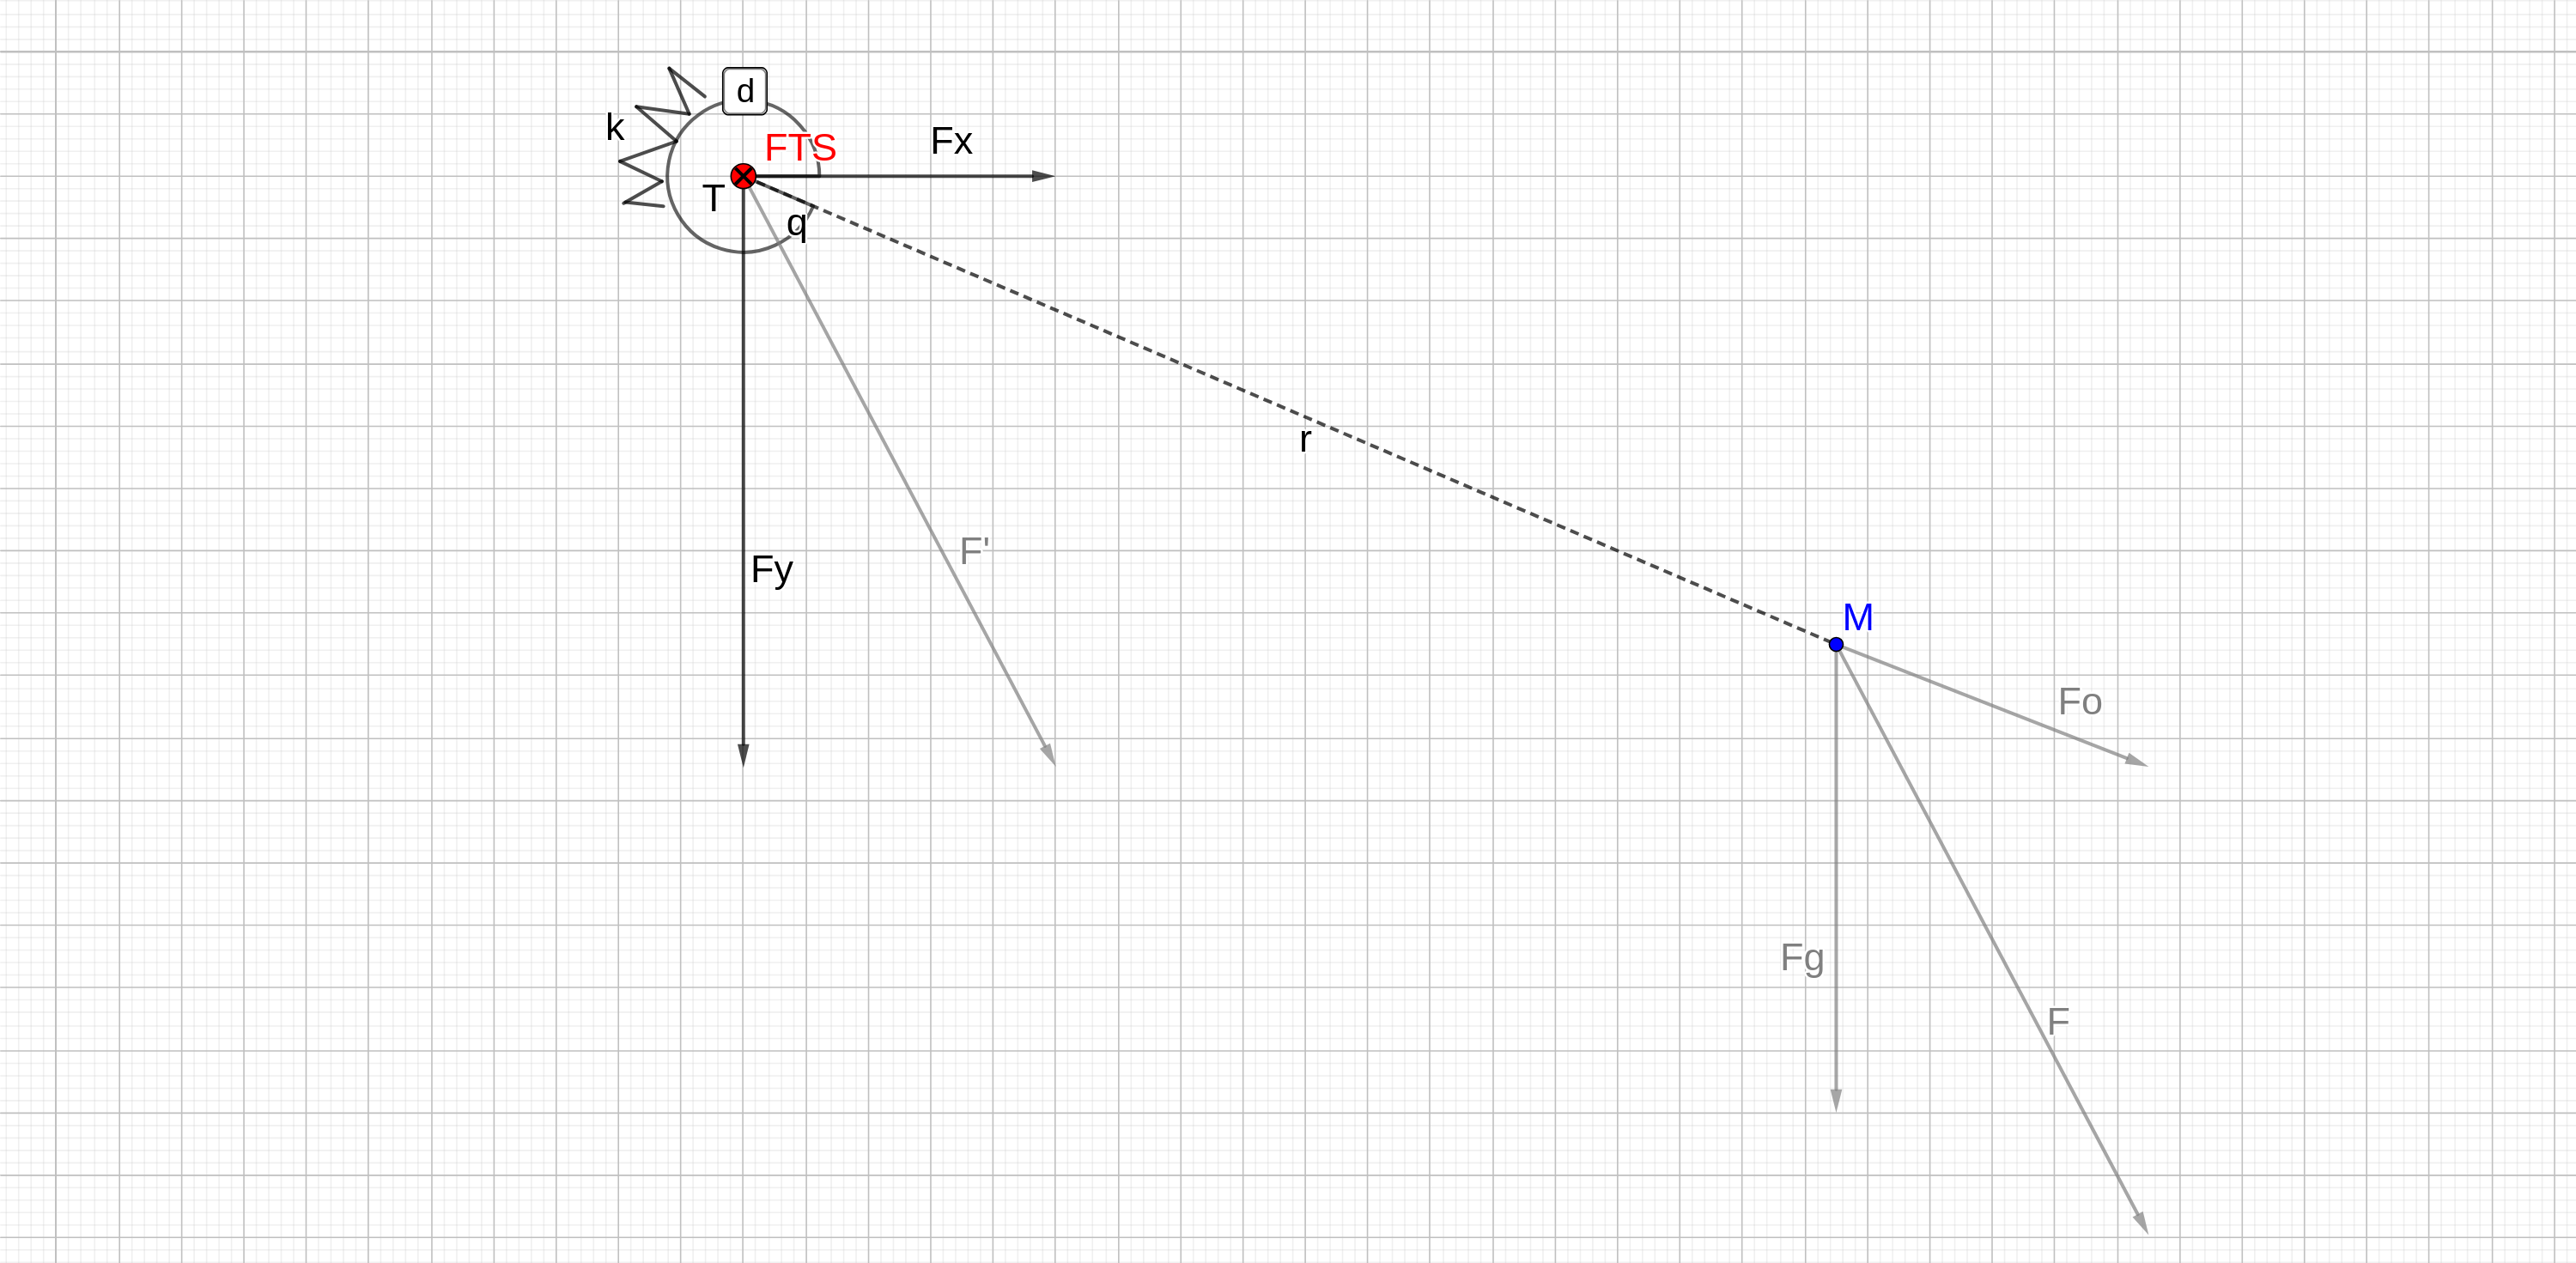
\includegraphics[scale=1.30]{2d}
\end{figure}
\framebreak
\begin{equation}
	\tau = I\ddot{q} = mr^2\ddot{q} = kq + d\dot{q} + mgr\cos{(q)} + Iu
\end{equation}
\begin{equation}
	\begin{bmatrix}
	    \dot{q} \\
	    \ddot{q}
	\end{bmatrix}
	=
	\begin{bmatrix}
	    0 & 1 \\
	    \frac{k}{I} & \frac{d}{I}
	\end{bmatrix}
	\begin{bmatrix}
		q \\
	    \dot{q}
	\end{bmatrix}
	+
	\begin{bmatrix}
	    0 \\
	    \frac{1}{I}
	\end{bmatrix}
	(mgr\cos{(q)} + \tau_u)
\end{equation}

W podejściu macierzowym mamy:
\begin{equation}
\mathbf{A} = 	\begin{bmatrix}
	    0 & 1 \\
	    \frac{k}{I} & \frac{d}{I}
	\end{bmatrix}
\end{equation}
\begin{equation}
\mathbf{B} = \begin{bmatrix}
	    0 \\
	    1
	\end{bmatrix}
\end{equation}

\begin{equation}
F_{y}(t)  = m(g + \dot{q(t)}^2r\sin{(q(t))})
\end{equation}

\end{frame}

\begin{frame}{Symulacja}
Po zdyskretyzowaniu metodami ZOH:
\begin{equation}
q(t+1) = \mathbf{A_d}q(t) + \mathbf{B}_du(t)
\label{eq:dyskretny}
\end{equation}

Po zdyskretyzowaniu metodą Eulera:
\begin{equation}
F_{y}(t) = mg + \sin{(q)}m(\frac{q(t)-q(t-1)}{T})^2 r
\end{equation}

\begin{equation}
\tau(t) = kq(t) + d\frac{q(t)-q(t-1)}{T} + I\tau_u(t) + \cos(q(t))mg
\end{equation}
\end{frame}

\begin{frame}{Zadanie optymalizacji}
\begin{equation}
\begin{aligned}
& \underset{m, r, I}{\text{min}}
&  \sum_{k=1}^{n} || e(t) || = \sum_{k = 1}^{n} || \begin{matrix}
\hat{F_y(t)}-F_y(t) \\
\hat{\tau(t)}-\tau(t) \\
\end{matrix} || \\
& \text{przy ograniczeniach:}\\
& & F_{y}(t) = m(g + \dot{q(t)}^2r\sin{(q(t))})\\
& & \tau(t) = I\ddot{q(t)}^2\\
\end{aligned}
\end{equation}

Zadanie jest rozwiązywane algorytmem Levenberga-Marquardta.
\end{frame}

\begin{frame}{Algorytm kompensacji}
Chcemy wyeliminować ten człon systemu:
\begin{equation}
	\begin{bmatrix}
	0 \\
	\frac{1}{I}
	\end{bmatrix}
	(mgr\cos{(q(t))} + \tau_u(t)) = 	\begin{bmatrix}
	0 \\
	0
	\end{bmatrix}
\end{equation}

Możemy przyjąć sterowanie:
\begin{equation}
\tau_u(t) = -\frac{mgr\cos{(q(t))}}{I}
\end{equation}

W celu zapobiegania gwałtownych zmian systemu algorytm załączamy z funkcją aktywacji.
\end{frame}

\begin{frame}[allowframebreaks]{Wynik eksperymentu}
\begin{figure}
	\centering
	\begin{subfigure}{.5\textwidth}
		\centering
		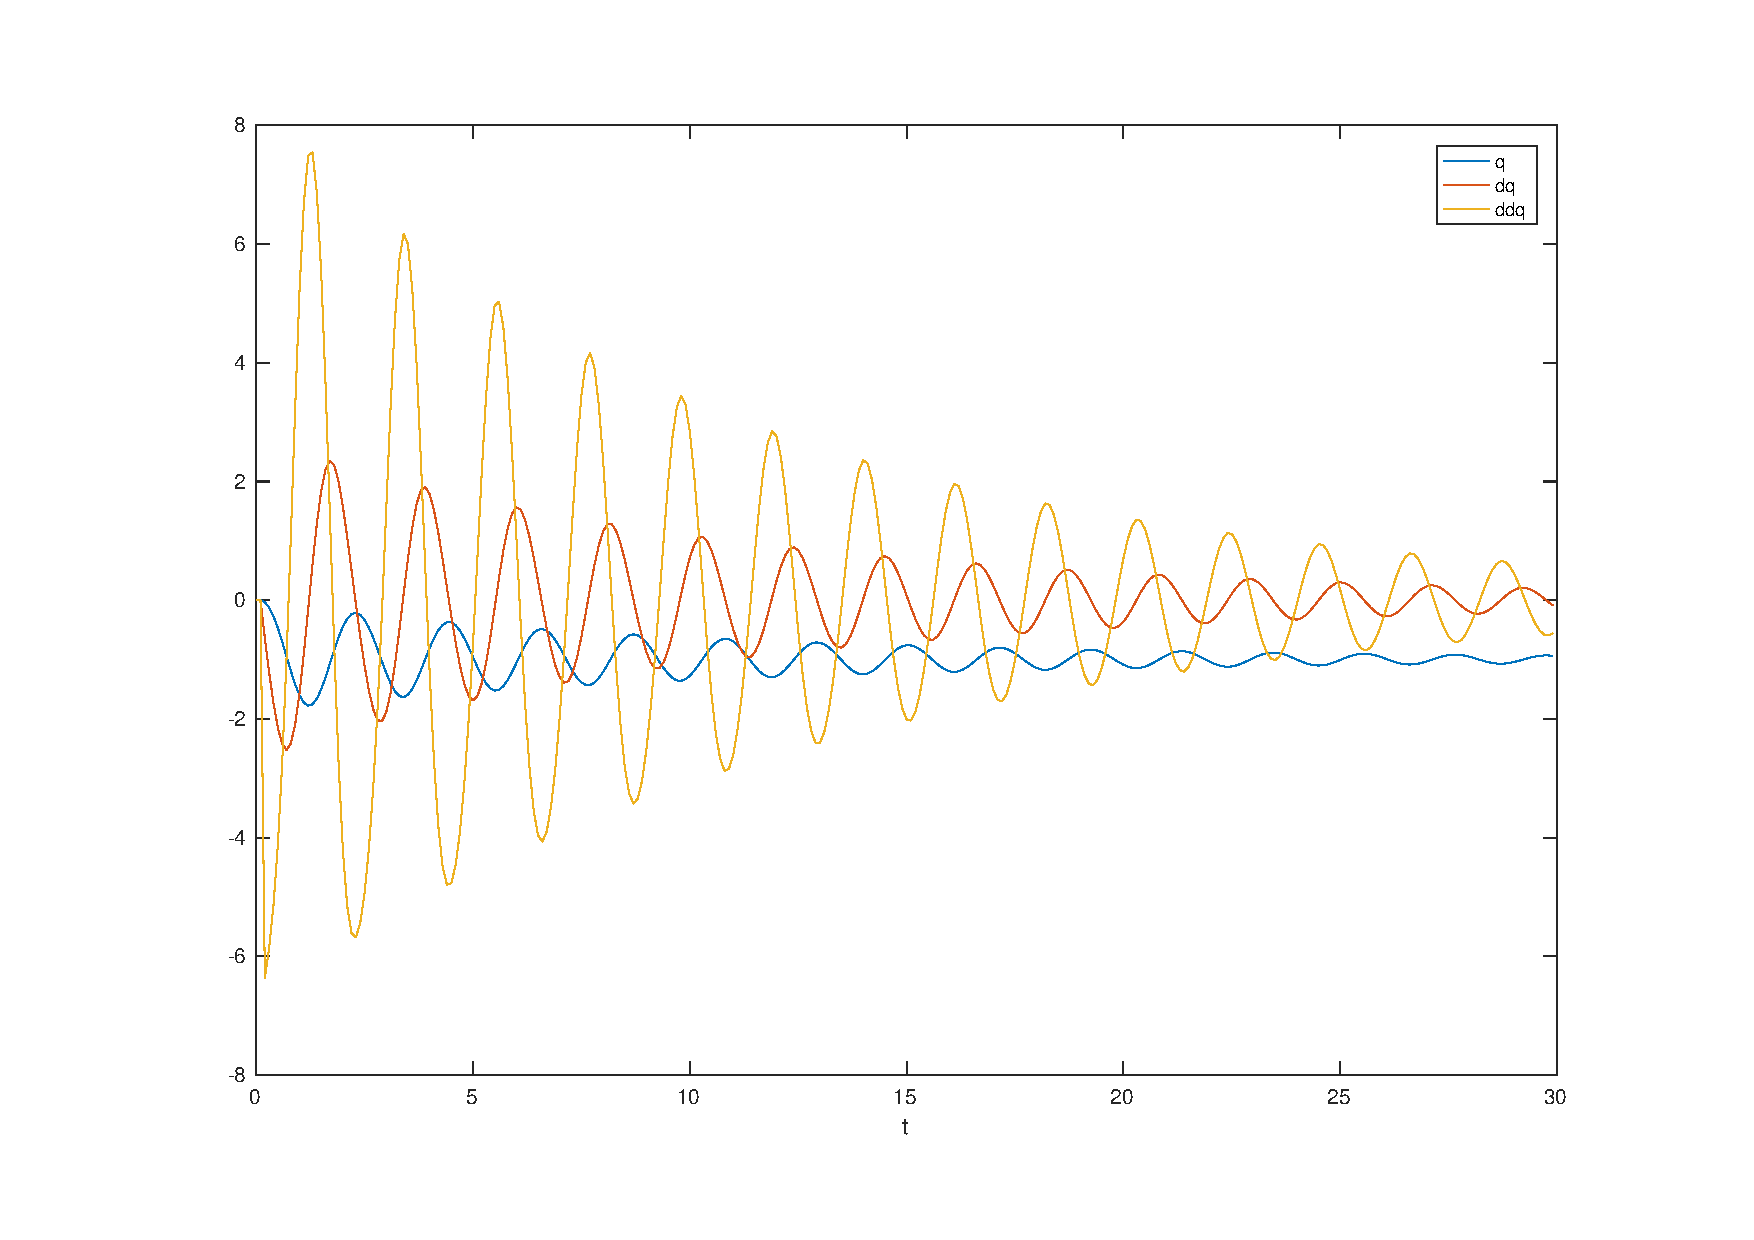
\includegraphics[width=\linewidth]{test_p}
	\end{subfigure}%
	\begin{subfigure}{.5\textwidth}
		\centering
		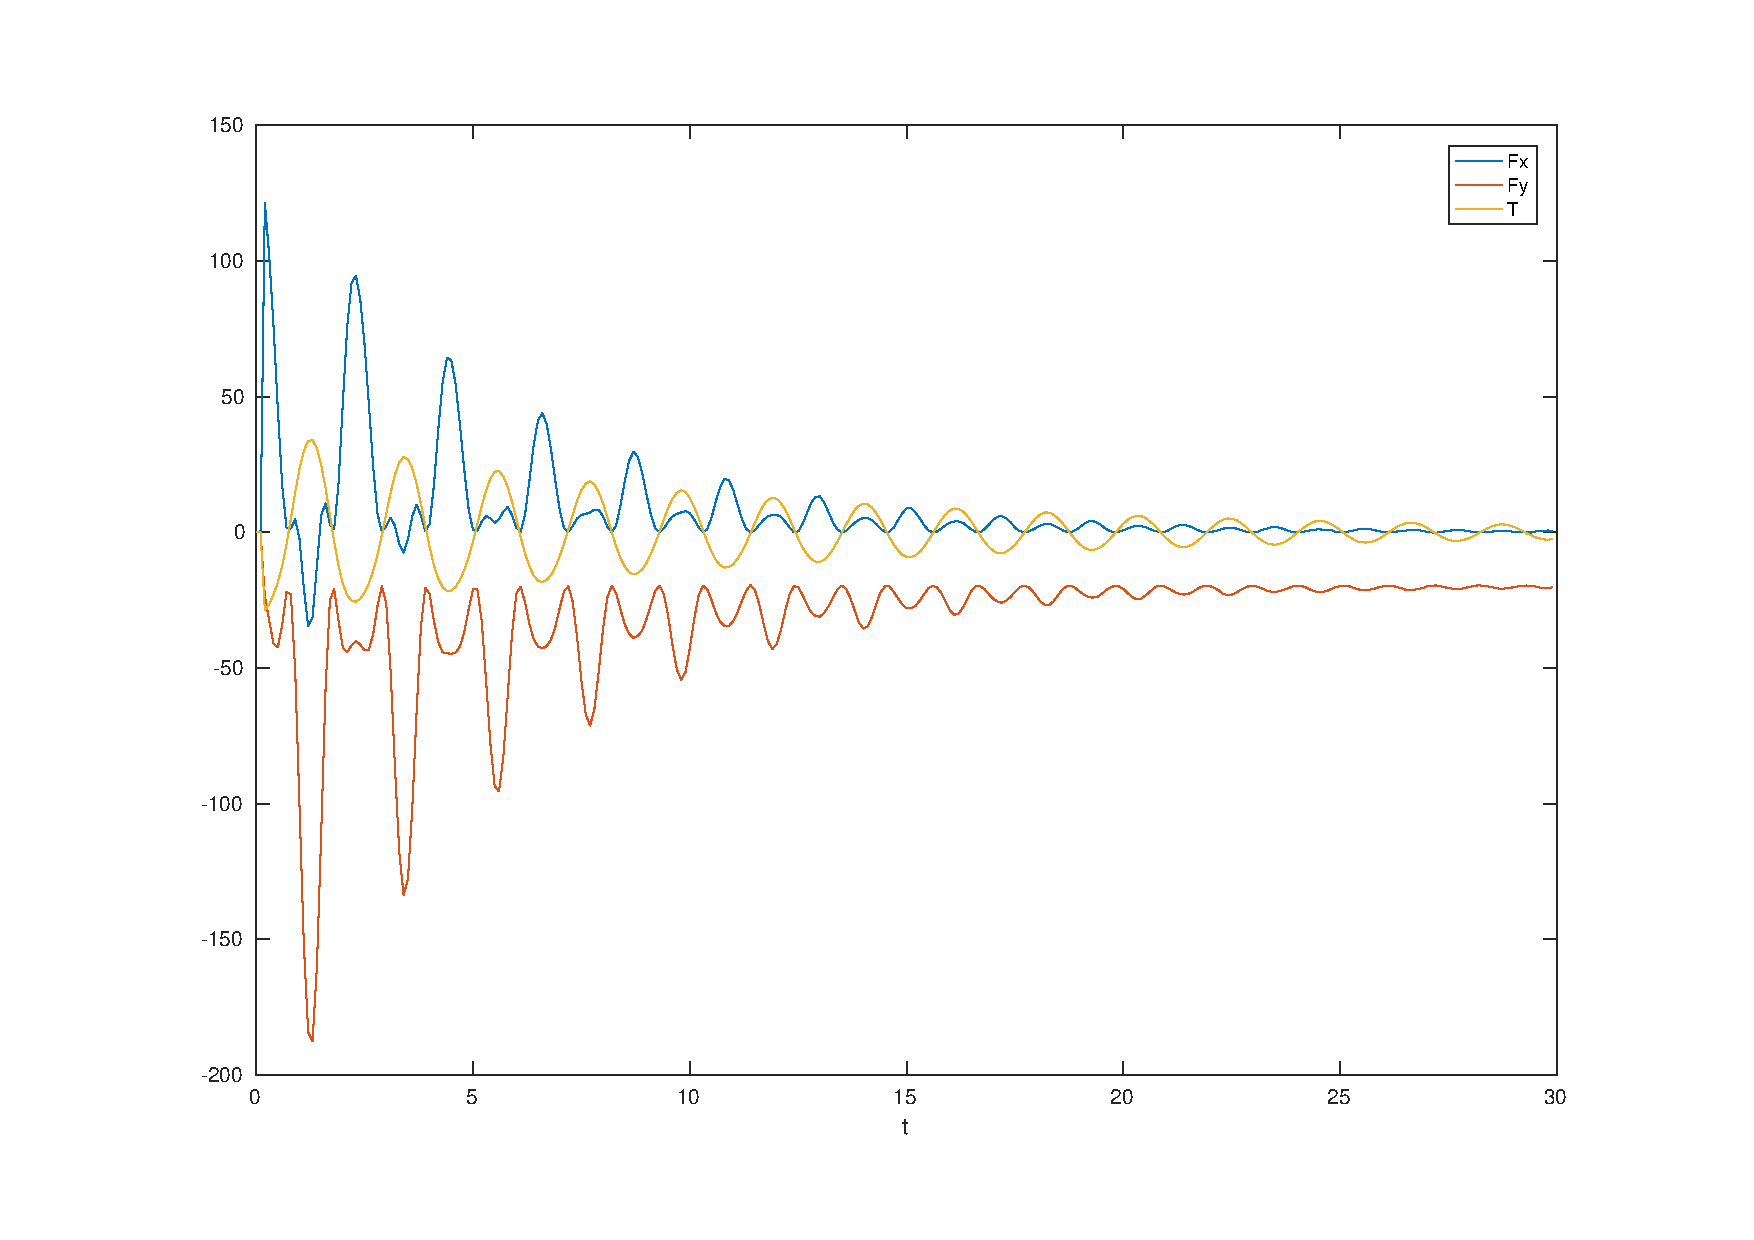
\includegraphics[width=\linewidth]{test_s}
	\end{subfigure}

	\caption{Symulacja układu z parametrami $T=0.01$, $m = 2$, $r = 1.5$, $k = 16$, $b = 2$. Brak kompensacji grawitacji.}
	\label{fig:system}
\end{figure}

\framebreak

\begin{figure}
	\centering
	\begin{subfigure}{.5\textwidth}
		\centering
		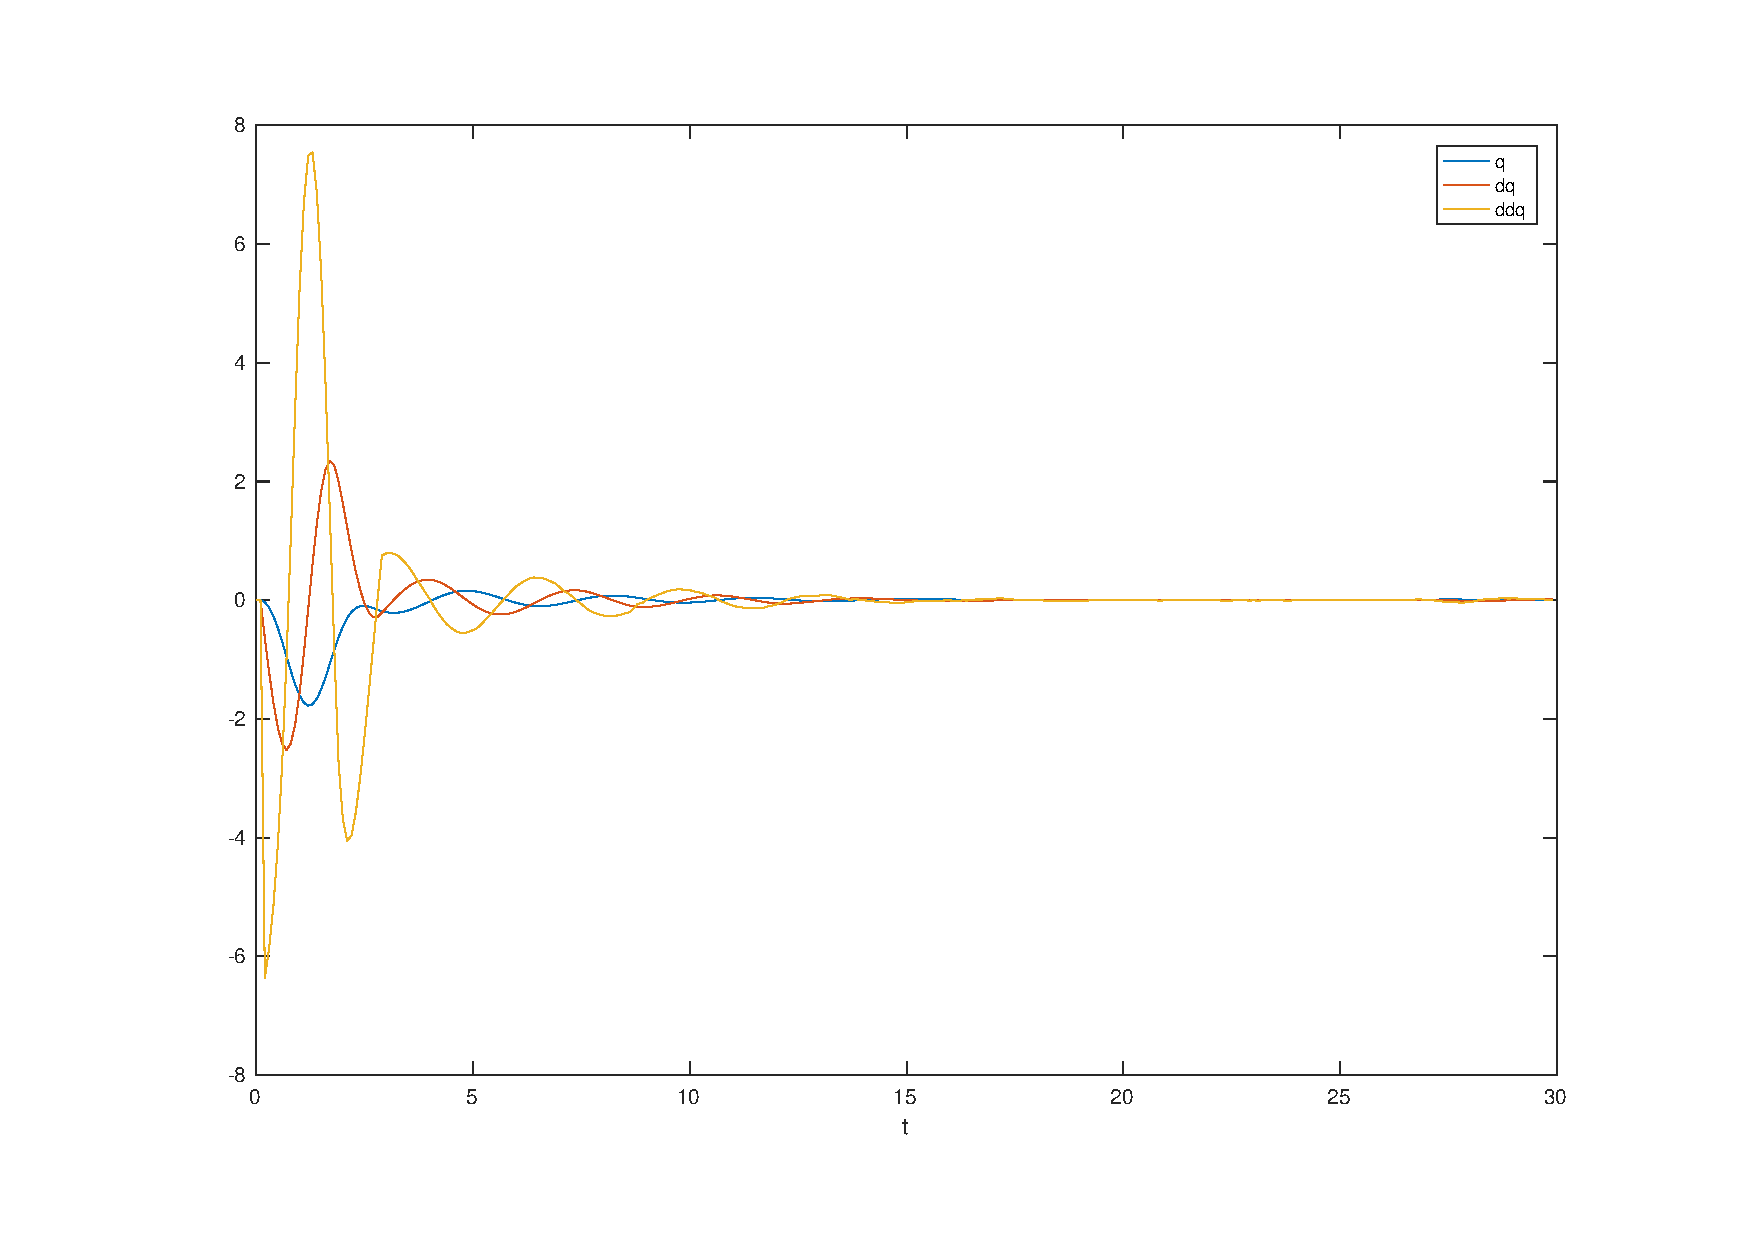
\includegraphics[width=\linewidth]{mrozenie_p}
	\end{subfigure}%
	\begin{subfigure}{.5\textwidth}
		\centering
		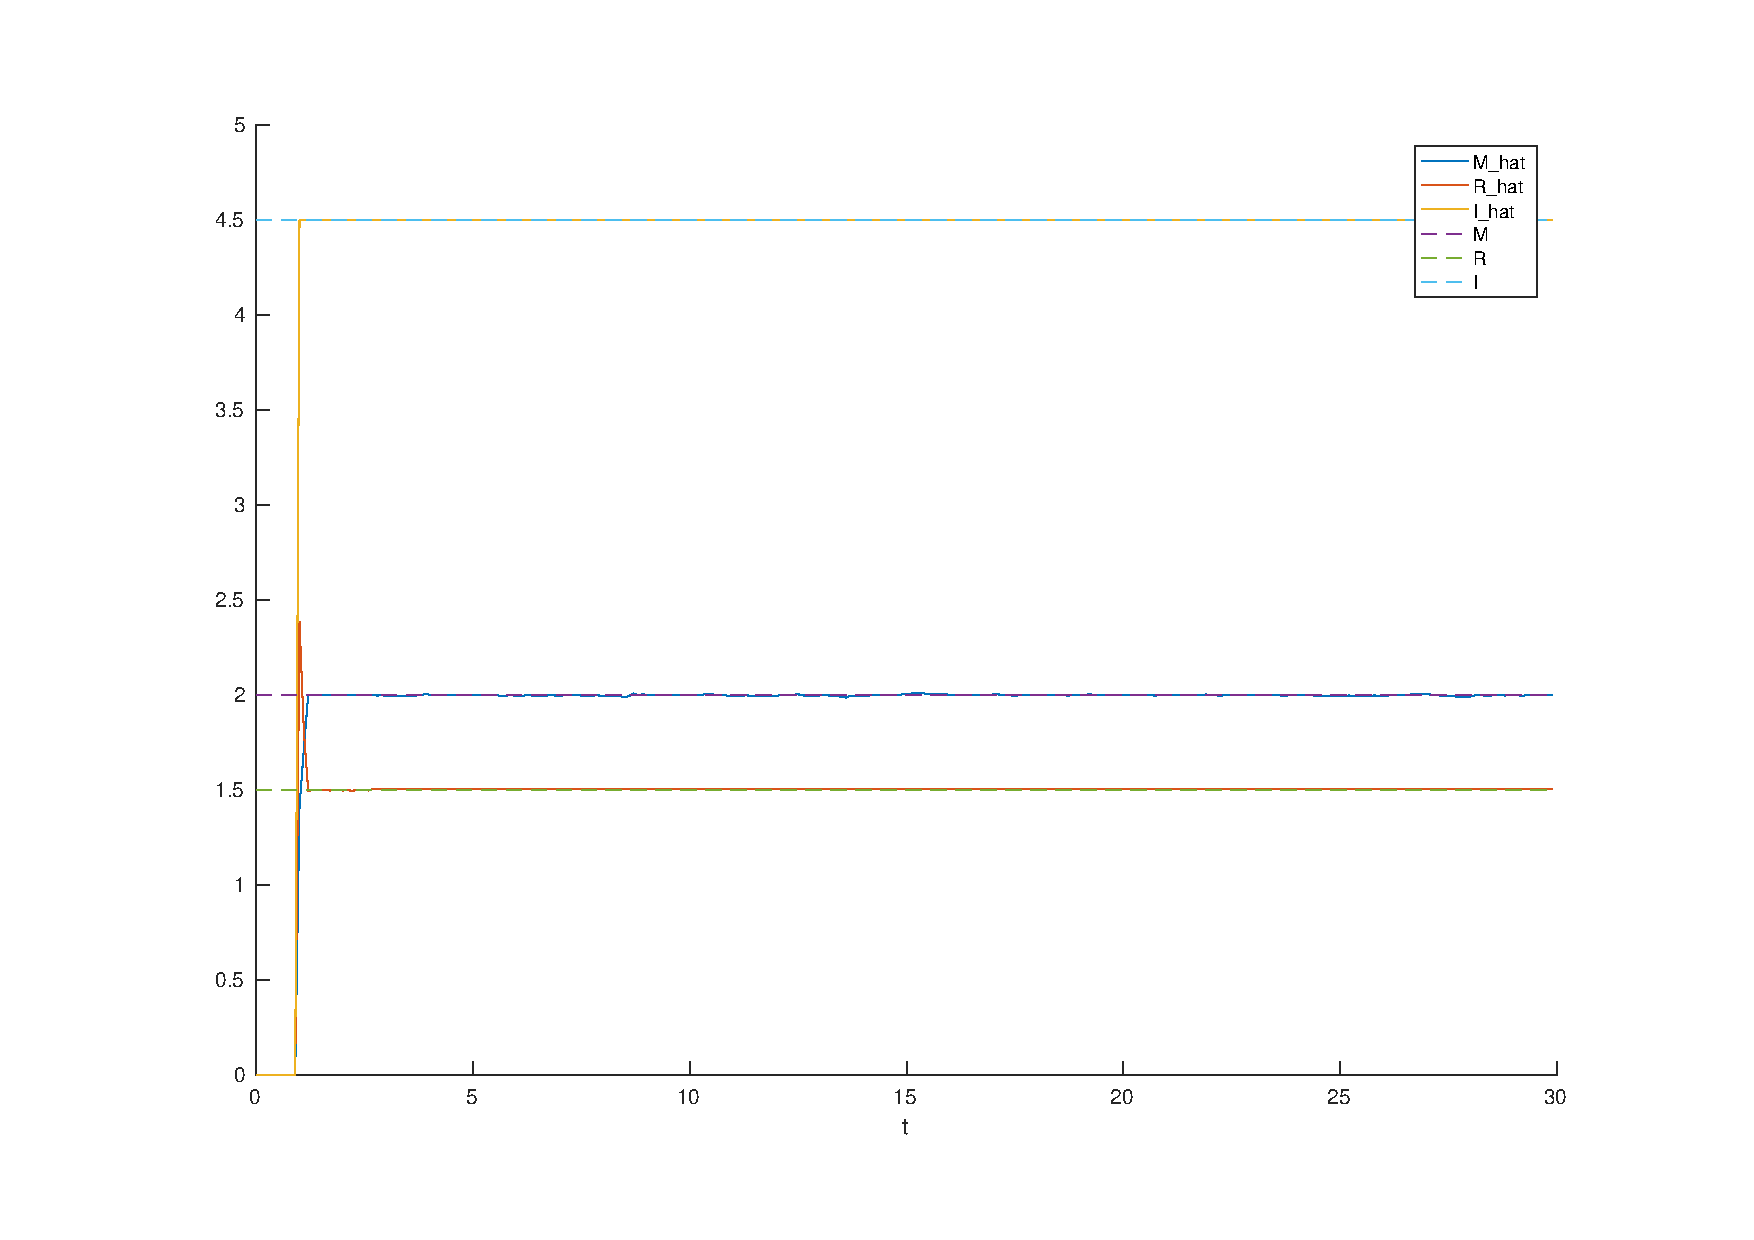
\includegraphics[width=\linewidth]{mrozenie_c}
		\label{fig:mrozenie_c}
	\end{subfigure}%

	\begin{subfigure}{.5\textwidth}
		\centering
		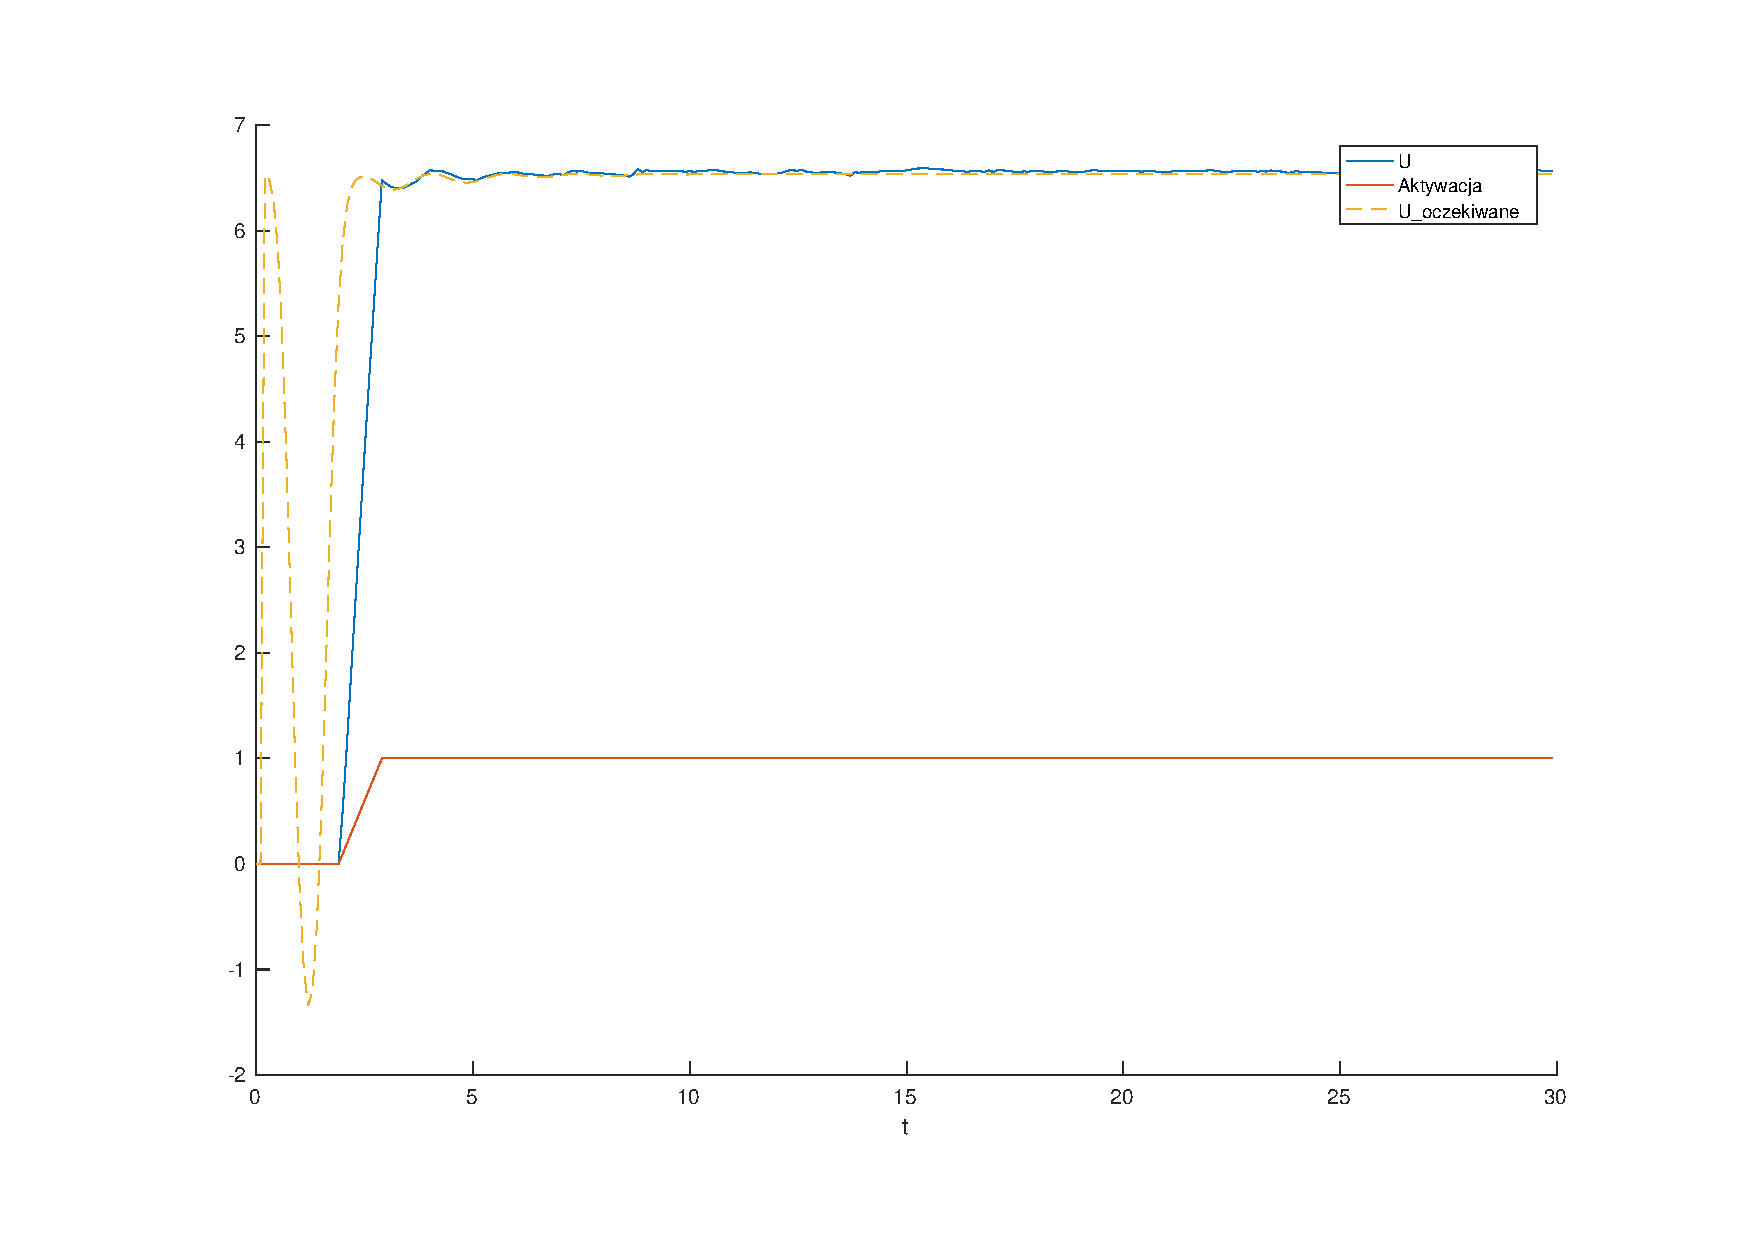
\includegraphics[width=\linewidth]{mrozenie_u}
		\label{fig:mrozenie_u}
	\end{subfigure}

	\caption{Symulacja układu z parametrami $T=0.01$, $m = 2$, $r = 1.5$, $k = 16$, $b = 2$. Załączona kompensacja grawitacji.}
	\label{fig:mrozenie}
\end{figure}
\end{frame}

\section{Podsumowanie}
\begin{frame}{Bibliografia}
\begin{itemize}
	\item Task-level approaches for the control of constrained multibody systems. \textit{Vincent De Sapio, Oussama Khatib, Scott Delp}.
	\item System identification: Theory for thee User. \textit{Lennart Ljung}
	\item \url{https://studywolf.wordpress.com/2013/09/07/robot-control-3-accounting-for-mass-and-gravity/}
	\item Modelling and Control of Robot Manipulators. \textit{L. Sciavicco, B. Siciliano}
	\item Część wiedzy pochodzi z artykułów zespołu np.: Two Mode Impedance Control of Velma Service Robot Redundant Arm.
	\textit{Tomasz Winiarski, Konrad Banachowicz, Dawid Seredyński}.
	\item Niektóre zdjęcia pochodzą ze strony \url{https://robotyka.ia.pw.edu.pl}

\end{itemize}

\end{frame}
\begin{frame}{Dziękuję za uwagę}
%\begin{figure}[h]
%	\centering
%	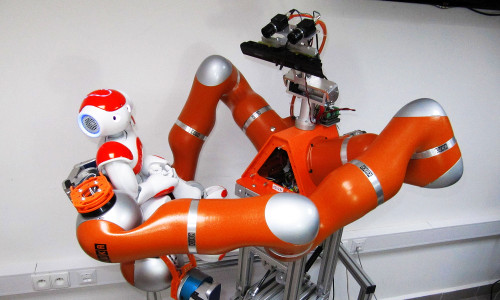
\includegraphics[scale=1.4]{velma3}
%\end{figure}
\end{frame}
\end{document}